\documentclass[12pt]{article}
\usepackage[top=1.5cm,bottom=1.5cm,right=2.5cm,left=2.5cm]{geometry}
\usepackage[francais]{babel}
\usepackage[utf8]{inputenc}
\usepackage[T1]{fontenc}
\usepackage[absolute]{textpos} 
\usepackage{graphicx}
\usepackage{caption}
\usepackage{amsthm}


\title{Rapport du TER}

\theoremstyle{plain} \newtheorem{theoreme}{théorème}

\begin{document}
\vspace{10mm}
\def\blurb{%
   Université des Sciences de Montpellier \\
  Master 1 Semestre 2 \\
  Unité d'Enseignement FMIN205 \\
  Site Internet : http://mus-d.lydiman.net/
	}
\def\clap#1{\hbox to 0pt{\hss #1\hss}}%
\def\ligne#1{%
  \hbox to \hsize{%
    \vbox{\centering #1}}}%
\def\haut#1#2#3{%
  \hbox to \hsize{%
    \rlap{\vtop{\raggedright #1}}%
    \hss
    \clap{\vtop{\centering #2}}%
    \hss
    \llap{\vtop{\raggedleft #3}}}}%
\def\bas#1#2#3{%
  \hbox to \hsize{%
    \rlap{\vbox{\raggedright #1}}%
    \hss
    \clap{\vbox{\centering #2}}%
    \hss
    \llap{\vbox{\raggedleft #3}}}}%
\begin{document}
\thispagestyle{empty}\vbox to 1\vsize{%
  \vss
  \vbox to 1\vsize{%
    \haut{}{\blurb}{}
    \vfill
    \ligne{\Large \maketitle{}}
   % \vspace{5mm}
    \ligne{}
    \vfill
    \ligne{%
     }
    \vspace{15mm}
    \ligne{%
      \begin{tabular}{l}
        Romain \textsc{Maneschi}\\
        Audrey \textsc{Novak} \\
	Jonathan \textsc{Fhal}\\
	Mélanie \textsc{König} \\
	Laurent  \textsc{Maillet}
      \end{tabular}
      }
    }%
  \vss
  }

\newpage

\tableofcontents

\newpage

\section{Introduction}
	\subsection{Généralités}
	Ce projet est réalisé dans le cadre de l'unité d'enseignement TER, en première année de Master Informatique à l'université des Sciences de Montpellier. Il a été proposé et encadré par le professeur Christophe Dony. Notre groupe est composé de 5 étudiants. \\
	\indent Ce projet consiste à créer un ensemble de classes qui permettra de programmer plus facilement des jeux de type "arcade". Ces jeux pourront être utilisés sur Internet, quelque soit le navigateur et le système d'exploitation de l'utilisateur. En outre ils pourront également tourner directement dans le système de l'utilisateur.
	
	\subsection{Fonctionnalités et contraintes }
	Avec l'aide de notre framework, un utilisateur pourra facilement créer des jeux d'arcades et donner aux objets qu'ils contiennent des comportements courants dans ce type de jeux tels que la collision par exemple. \\
	\indent La principale contrainte que nous imposait le sujet était que l'utilisateur puisse programmer un petit jeu d'arcade en quelques lignes, ou tout du moins en peu de temps et ceci en étendant simplement les classes de notre framework. La seconde contrainte était que les jeux créés à l'aide du framework puisse être utilisable sur Internet. \\
	\indent De plus, afin de mettre en pratique nos cours d'UML, mais surtout pour bénéficier d'une architecture de classes claire et facilement maintenable, nous avons décidé d'implémenter nos classes sous la forme du modèle MVC.

	\subsection{Quelques définitions}
	Avant de commencer à présenter notre framework, il nous parait important de rappeler quelques définitions :
	
		\subsubsection{Bibliothèque Logicielle}
		Egalement appelée librairie, une bibliothèque logicielle est constituée d'un ensemble de fonctions qui pourront être utilisées sans avoir à les réécrire. Ces fonctions sont la plupart du temps regroupées par thèmes.

		\subsubsection{Ligne de produits}
		Une ligne de produits est un ensemble de produits mis à disposition par une entreprise pour répondre à un même besoin, ou ayant des caractèristiques communes. Elle permet également d'augmenter la productivité tout en diminuant le temps et donc le coût de réalisation du produit. \\ \\
		\indent \textbf{Ligne de produits logiciels} \\
			\indent Ensemble de logiciels appartenant à un domaine particulier, ici la création de jeux d'arcades. En informatique une ligne de produits est également appelée un framework. Généralement, un framework est codé dans un langage objet, par conséquent il est composé d'une classe mère de laquelle découle plusieurs classes filles. Ainsi un programmeur doit réimplémenter les classes qui l'intéressent pour créer son logiciel. \\
		\indent Une ligne de produits logiciels est une surcouche des bibliothèques et permet donc non seulement de pouvoir réutiliser du code mais aussi et surtout de donner une architecture précise aux logiciels qui l'utilisent. De plus un framework doit être nécessairement extensible pour s'adapter à un plus grand nombre de logiciels.
		\subsubsection{Jeux d'Arcades}
		Les jeux d'arcades sont principalement des jeux à deux dimensions. La jouabilité est très simple ce qui rend ce type de jeux très populaires. Il n'y a généralement pas d'intelligence artificielle (ou très peu évoluée) et encore moins de parties réseaux (les joueurs s'affrontent sur la même machine). \\
		\indent A l'origine ce type de jeux à été créé pour les salles de jeux ou certains bars, c'est pour cela que le niveau du jeu est exponentiel, afin que le joueur remette en permanence de l'argent pour faire vivre son personnage. Ceci explique aussi le fait qu'il n'y ait pas de sauvegardes des parties. \\
		\indent Quelques exemples de jeux bien connus : Pac-Man, Casse-Briques, Ping-pong...

	\subsection{Outils utilisés}
		\subsubsection{Choix du langage}
		\indent Ce projet impose de pouvoir utiliser cette ligne de produits pour créer nos propres jeux d'arcades. Ces jeux doivent être jouables sur Internet. De nos jours il n'existe pas beaucoup de langages de programmation permettant cela. Les deux plus répandus sont JavaScript et Flex. Flex étant un tout nouveau langage développé par Adobe, il nous à paru intéressant de le découvrir et d'exploiter sa richesse plutôt que de réutiliser un langage connu de tous : JavaScript.
		\subsubsection*{ActionScript}
			\indent L'ActionScript est le langage propriétaire d'Adobe, développé dans le but de contrer JavaScript. La syntaxe est très proche de JavaScript et permet de faire des applications orientées objet.
		\subsubsection*{Flex}
			\indent Ce nouveau langage basé sur ActionScript permet de créer des clients internets riches avec une syntaxe à balises. Ainsi les scripts écrits en Flex sont transformés en ActionScript puis compilés en SWF (format propriétaire d'Adobe également appelé Flash). Ainsi tout navigateur équipé de Flash peut lire les applications Flex.
			\ident Nous avons donc créé notre framework en ActionScript, car c'est un langage objet, actuellement en version 3 (donc stable et évolué). Cela laisse donc le choix aux utilisateurs de notre framework de réimplémenter nos classes en ActionScript ou de développer directement leurs applications en Flex.
			\ident L'inconvénient de ce choix est que toute la technologie est propriétaire. Il faudra donc que l'utilisateur final ait tous les outils nécessaires à la programmation et surtout compilation de Flex.
		\subsubsection{IDE}
		\indent Adobe a fait le choix de ne pas développer d'IDE spécialisé pour son langage, préférant utiliser Eclipse par le biais d'un plugin. Eclipse est un IDE très populaire car libre de droit et très performant puisqu'en version 3. Nous ne sommes donc pas perdus puisque nous avons l'habitude de développer avec cet IDE.
		\subsubsection{Google Code}
		\indent Pour pouvoir travailler en groupe nous avons eut besoin d'un site internet pour regrouper nos codes et nos idées. Google Code est une plate-forme nous offrant un Wiki pour échanger nos idées, un serveur SVN pour partager nos sources, un espace de stockage de fichiers et enfin un contrôleur de bugs afin d'être prévenu d'éventuels problèmes.
		\ident De plus il est entièrement gratuit et est hébergé chez Google, ce qui nous assure une plus grande sérénité quand à la sauvegarde de nos données.
		\subsubsection{SVN}
		\indent Puisque Google nous offre un serveur SVN nous l'utilisons pour garder la même version pour chacun des développeurs. 
		\ident Sous Linux nous utilisons le client RapidSvn pour sa simplicité (un tutorial sur son utilisation est disponible sur le site du projet).
		\ident Sous Windows nous utilisons Tortoise pour les mêmes raisons.
		\subsection{Modélisation UML}
		\indent Nous utilisons le logiciel BOUML pour modéliser l'architecture du framework car il est simple d'utilisation, multi-plateforme et gratuit.

	\subsection{Organisation}
		\subsubsection{Répartition des tâches}
			La répartition des tâches s'est éffectuée selon les préférences de chacun.
			\begin{itemize}
				\item Maneschi Romain (chef de groupe) : Partie graphique
				\item Maillet Laurent : Code métier 
				\item König Mélanie : Contrôleurs, effets et collisions
				\item Novak Audrey : Créateur de jeux
				\item Fhal Jonathan : Création de jeux utilisant le framework
			 \end{itemize}
			
%		\subsubsection{Diagramme de Gantt}
%			Nous prévoyons de suivre cette ligne de conduite :
			\begin{center}
				\begin{textblock*}{19cm}(1.5cm,16cm) 
			%		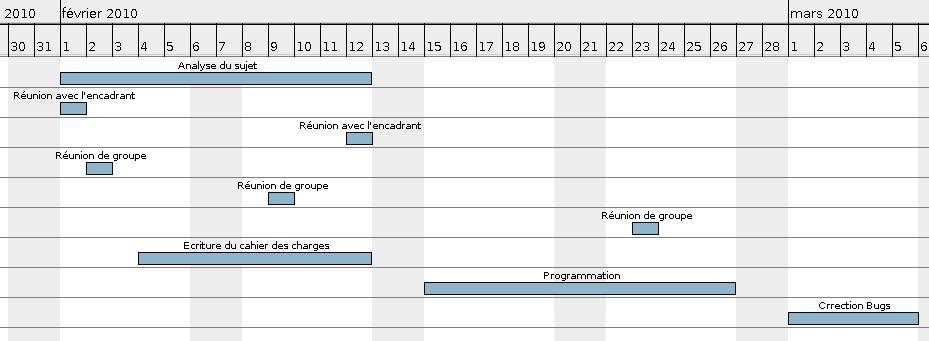
\includegraphics[width=1.00\textwidth]{diagramme-gantt.jpg}
				\end{textblock*}		
			\end{center}

\newpage	
\section{Code métier}
	La partie la plus importante de tout framework -et même de toute application fonctionnelle- réside dans la qualité d'implémentation du code métier. Plus le code métier d'un framework sera à la fois facile de compréhension et d'accès, réutilisable tout en restant léger et puissant, plus le framework sera rapide et offrira de nombreuses possibilités. C'est pourquoi nous avons décidé de consacrer la plus grosse partie de notre travail sur le coeur de notre framework.
	\\ \\
	\indent Après une analyse attentive du problème que pose la réalisation d'un framework de jeu, nous avons rapidement pu construire une représentation interne du framework et ainsi décider des designs pattern qui seraient les mieux adaptés à sa réalisation.

	\subsection{Le pattern MVC}
		\begin{center}
			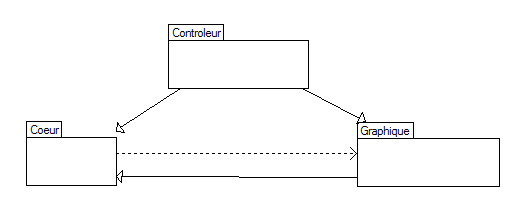
\includegraphics[width=1.0\textwidth]{img/MVC.png}  
			\caption{Modèle Vue Contôleur}
			\label{cas_utilisation}			
		\end{center}
	
	\indent Avant toute chose, il nous a paru évident de bien différencier les représentations que l'on devait faire de chaque objet de notre framework. En effet dans un jeu, un objet possède une représentation graphique ainsi qu'une représentation interne (les données de l'objet en question). De plus il peut être nécessaire de vouloir qu'une action dirigée par un utilisateur permette d'avoir des effets sur notre objet, tant bien au niveau graphique, qu'au niveau des données de l'objet. Il nous a alors paru évident que nous devions nous inspirer du modèle MVC pour réaliser notre framework.
	\\ \\
	\indent Pour tout objet du framework il a donc été nécessaire de représenter en deux parties différentes tout objet : d'un coté le graphisme (voir le package Graphique) et de l'autre les données (voir le package Coeur). Pour permettre de relier les deux parties d'un objet, il a fallu installer le graphisme en position d'écouteur du coeur. Ainsi lorsque les données du coeur d'un objet sont modifiées, le graphisme en est immédiatement informé et peut réagir en conséquence.
	\\ \\
	\indent Les controleurs, qu'ils soient de type effet, souris ou clavier, agissent sur un objet du code métier en modifiant les propriété de ceux-ci. Ces modifications seront répercutées sur le graphisme puisqu'il est écouteur de la partie métier.
% laurent
\newpage
	\subsection{Objets}
\\	
	\begin{textblock*}{14cm}(2cm,2.5cm)
		\begin{center}  
			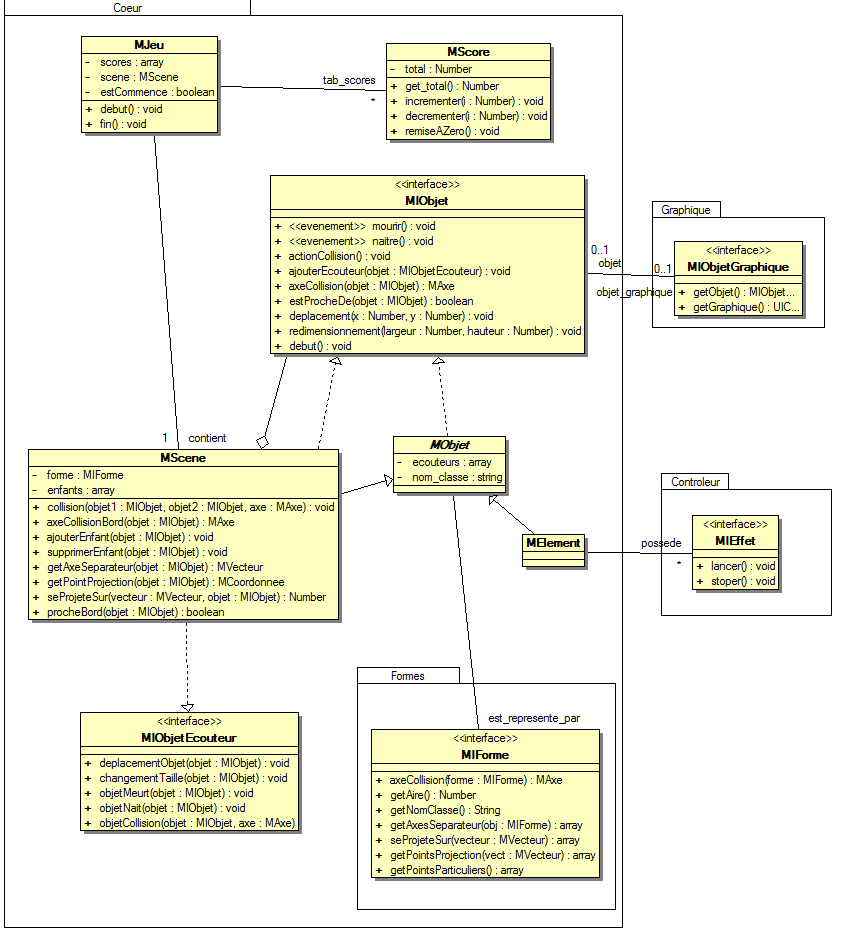
\includegraphics[width=1.4\textwidth]{img/Coeur_7.png} 
			\caption{Diagramme de classe du coeur}
		\end{center}
	\end{textblock*}
\newpage	
	L'architecture la plus logique pour les objets aurait été une interface avec toutes les fonction nécéssaire dans nos objets et une classe abstaite implémentant cette interface en redéfinissant les fonctions communes à tous les objets. Malheureusement, nous nous sommes heurté à la première limitation de notre langage, les classes abstraites ne sont pas implémentables en Actionscript 3. Nous avons créé une interface MIObjet représentant l'ensemble des fonctionnalités nécessaires à la bonne implémentation d'un objet. A partir de cela nous avons créé une classe "abstraite" MObjet, implémentant la plupart des fonctions demandées par l'interface. Nous avons pensé que certaines fonctions sont génériques à tous les objets -par exemple changer les coordonnées de l'objet- alors que d'autres nécessitent d'être forcément spécifiées. A la construction d'un MObjet nous avons forcé le fait que les utilisateurs du framework doivent implémenter MIObjet. Ainsi grâce à cette implémentation, nous forçons les utilisateurs qui veulent étendre la classe MObjet à implémenter MIObjet, ce qui permet de ne pas nuir au bon fonctionnement de notre framework.
	\\ \\
	\indent Deux types d'objets nous ont paru essentiels pour créer la base de n'importe quel jeu : les scènes et les éléments. A partir de la hiérarchie d'objets de base, nous avons donc créé ces deux nouveaux types d'objets.
	\\
	\indent	Une scène est un objet sur lequel l'utilisateur n'est pas censé pouvoir effectuer d'action de base comme le déplacement (cela reste possible cependant mais pas forcément intéressant), mais c'est un objet pouvant contenir d'autres objets afin qu'en son intérieur se déroulent des actions (comme des déplacements ou des collisions). Nous avons mis en place un "composit pattern" : une scène est un objet contenant d'autres objets.
	\\
	\indent Un élément est un objet de base auquel on rajoute une liste d'objets qui l'écoutent et une liste d'effets. Les effets s'appliquent à tout moment sur un élément et permettent de lui donner vie (un déplacement perpétuel, changement de taille, etc.). Les éléments possèdent une liste d'effets afin de pouvoir combiner les différents effets possibles (agrandir l'élément tout en le déplaçant par exemple). 
	\\
	\indent Les objets qui écoutent les éléments doivent forcément être des objets implémentant l'interface MIObjetEcouteur. C'est grâce aux méthodes de cette interface que sont faites les liaisons entre les éléments et les écouteurs. En effet lors de certaines actions spécifiques telles que le déplacement, un élément va prévenir les objets qui l'écoutent qu'il s'est déplacé afin que ceux-ci puissent agir en conséquence.
	\\
	\indent Une scène est donc forcément un objet écouteur car elle doit savoir à tout moment ce qu'il se passe en elle : des objets se sont-t'ils rencontrés? un objet a-t-il touché le bord de la scène? Le joueur a t'il fini de casser toutes les briques de son casse-brique? Grâce à notre hiérarchie il devient facile de pouvoir répondre à toutes ces interrogations : la scène, lorsqu'elle reçoit un appel d'un des objets qu'elle contient, n'a qu'à agir en fonction.

\newpage
	\subsection{Eléments}
Après avoir réfléchi sur l'élément de base, un élément dont on peut positionner ses coordonnées, sa taille ou encore le fait qu'il puisse mourir, nous nous sommes intéressés à ce que pourrait vouloir faire un programmeur de jeux d'arcade. Avec notre élément de base et nos contrôleurs, il a déjà un large panel de possibilités et il peut quasiment tout faire mais notre but étant de lui faliciter la tâche au maximum, nous avons décidé d'ajouter plusieurs sous-éléments.
		
	\subsubsection{Patron de conception Etat}
Un programmeur pourrait vouloir positionner ses objets en tant qu'objet déplaçable ou non, redimensionnable ou non et enfin et surtout destructible ou pas. Pour faire cela nous avons décidé de mettre en place le patron de conception Etat. Certes tous ces états n'ont que deux possibilités, mais il y a plusieurs raisons à ce choix :
\begin{itemize}
	\item le programmeur peut vouloir changer d'état à tout moment
	\item un simple booléen aurait pu suffir mais les possibilités aurait alors été réduites
	\item cela permet de soulager la classe principale en déléguant du code à la classe représentant l'état
\end{itemize}

\indent Pour toutes ces raisons nous avons choisi d'implémenter le patron de conception état. 
		\begin{center}
			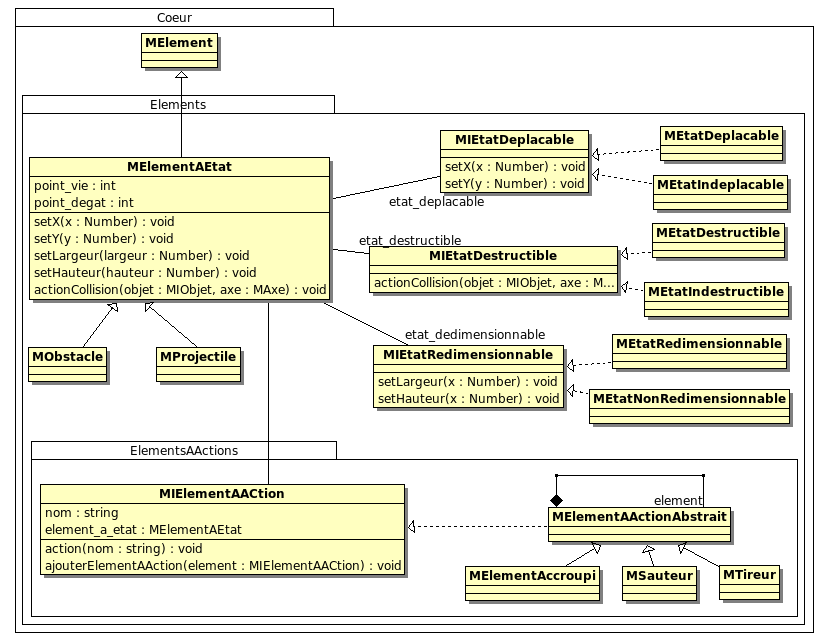
\includegraphics[width=1.00\textwidth]{img/Elements.png}
		\end{center}

	\indent La classe qui permettra tout ce processus est la classe MElementAEtat afin de ne pas toucher au code de la classe MElement qui est implémentée par un autre programmeur du groupe. De plus elle contient un attribut de chaque type : MIEtatDeplacable, MIEtatDestructible et MIEtatRedimensionnable qui représentent : les états pour le déplacement, la destruction ou encore le redimensionnement. Ainsi le programmeur peut facilement changer les caractéristiques de son élément en positionnant ses états en fonction par exemple d'objet bonus trouvés dans la scène.
\\\\
	\indent Ensuite nous nous sommes demandés quels types d'éléments nous pouvions construire à partir de ces états. Tout naturellement, nous avons immédiatement pensé aux obstacles implémentés par MObstacle qui est un élément indestructible et indéplaçable. Or, comme par définition il est indéplaçable, le programmeur ne pourrait plus le repositionner après l'avoir positionné une première fois sur la scène, afin d'éviter cela, nous le rendons indéplaçable seulement après avant fait appel à la fonction MJeu.getInstance.debut(). Ainsi si le jeu a commencé alors l'obstacle n'est plus déplaçable. 

\\
	\indent Puisque nous avons à notre disposition différents types de contrôles nous avons prévu une implémentation de base de ceux-ci :
\begin{itemize}
	\item par le clavier, c'est la première façon à laquelle on pense en tant que joueur. Ainsi nous avons implémenté la classe MControleClavier qui est un MElementAEtat implémentant MIEcouteurClavier avec les touches de base que tout le monde à l'habitude d'utiliser pour jouer : les flèches pour se diriger.
	\item par la souris, qui sert donc à diriger l'objet.
	\item enfin un programmeur peut vouloir qu'un élément soit contrôlé par le PC, autrement dit que celui-ci soit un ennemi du joueur. Pour cela nous avons mis en place un MMouvementPerpetuel dans le MElementAEtat. 
Enfin nous avons pensé aux projectiles, qui sont des éléments déplaçables et destructibles. Mais dès lors il faut pouvoir "tirer" ces projectiles de façon la plus simple possible.
\end{itemize}
		\subsubsection{Actions}
	L'étape suivante a été ensuite plus directement ciblée vers les jeux d'arcade de type "shoot". En effet, nous nous sommes rendus compte que nous pouvions accélérer considérablement le développement d'une telle application en créant et en associant un MProjectile à un "MTireur". Le problème étant qu'un élément qui est à état, controlé par le clavier, la souris ou encore un mouvement doit pouvoir tirer. Nous nous sommes donc dit que le fait de tirer doit venir "décorer" nos éléments. Ainsi nous avons mis en place le patron de conception "decorateur". Pour cela, une simple interface pour définir une action est requise, ensuite chaque action prend en paramètre l'élément qu'elle décore. Ce patern nous a ensuite permis d'imaginer ce qu'un développeur pourrait vouloir comme action, l'action de sauter est venue très rapidement ainsi que celle de s'accroupir. Nous aurions pû en implémenter plus mais le niveau actuel du graphique ne permettrait pas de les représenter. Mais notre framework étant extensible, elles seront facilement ajoutables ultérierement.

\newpage
	\subsection{Formes}
\\	
	 \begin{textblock*}{18cm}(1cm,2cm)  
		\begin{center}
			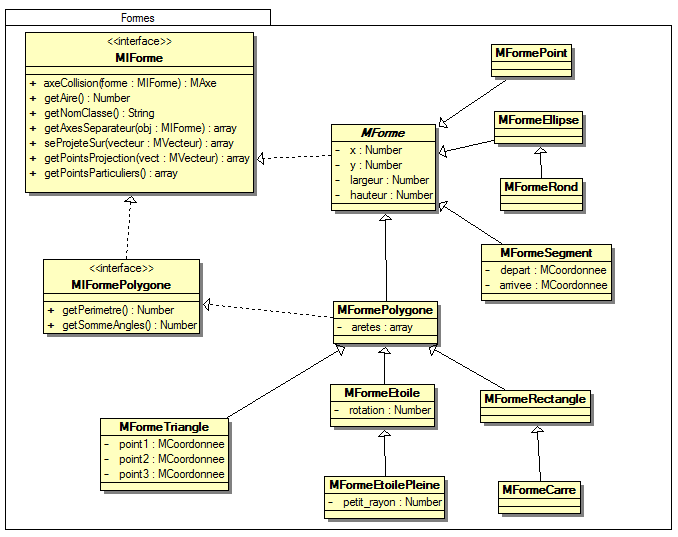
\includegraphics[width=1.1\textwidth]{img/Forme1.png} 
			\caption{Diagramme de classe des formes}	
		\end{center}
	\end{textblock*}	

\begin{textblock*}{18cm}(2cm,19cm)
	La réalisation des formes a été une partie importante de la réalisation des objets. Il est évident de penser que tout objet possède sa propre forme et que l'on voudra visuellement obtenir des rendus différents selon que l'on décide de créer des murs ou des balles. Dans le cadre de la réalisation de notre framework en suivant le pattern MVC, il a été obligatoire de procéder à deux types de représentations pour les formes : une graphique (présenté plus loin) et une dans le code métier. La partie graphique s'occupera uniquement du rendu à l'écran de la forme, alors que le coeur lui s'emploiera à conserver toutes les données de la forme.
	\\ \\
	\indent Lors de la réalisation des formes, nous avons rencontré le même problème que pour les objets : nous voulions créer une classe abstraite MForme abstraite reprenant toutes les fonctions et tous les attributs de base nécessaire à la création cohérente d'une forme. Nous avons du finalement opter pour la même solution que précédemment : une interface MIForme et une classe MForme reprenant toutes les fonctions de bases génériques à toutes les formes.
	\\
\end{textblock*}
\newpage
%	\\
	\indent On a distingué deux types de formes : les formes simples et les polygones. Toutes les formes sont caractérisées par des coordonnées x et y, ainsi que par une largeur et une hauteur. Ces quatre variables forment un rectangle dans lequel sera contenu la totalité de la forme, que ce soit une forme simple ou un polygone. \\
	\indent La différence entre les formes simples et les polygones réside dans le fait que les formes polygones ont besoin également d'un ensemble d'arêtes pour pouvoir être représentées. S'il est possible de représenter un triangle uniquement par des points, et de représenter un carré comme une forme simple, il devient beaucoup plus dur de représenter un polygone à n côtés uniquement par des points, ainsi que de représenter un carré pouvant tourner sur lui même uniquement à l'aide des quatre variables de base. Nous avons donc introduit des arêtes pour tout polygone ce qui permet de les dessiner et les représenter plus facilement.
	\\
	\indent Nous avons décidé de créer directement la plupart des formes de base ceci pour permettre à l'utilisateur de pouvoir créer des éléments directement sans avoir à tout implémenter. Ainsi s'il veut créer une balle il n'aura qu'à choisir une forme ronde représentée par la classe MFormeRonde.
	\\ \\
	
	\indent Enfin c'est dans les formes qu'une des plus dures parties du coeur a été géré : les collisions. En effet la collision s'effectue selon la forme d'un élément, comme nous allons vous l'expliquer maintenant.
	\subsection{Collision}
La détection de collision est l'un des plus importants aspects des jeux d'arcade, malheureusement elle est aussi souvent l'un de ses points faibles.\\
	\indent Quand il y a n objets distincts dans la scène, les tests doivent se faire entre O($n^{2}$) différentes paires d’objets, c’est-à-dire que si nous avons 10 objets, il faudra faire 10 * 10 = 100 tests. Nous avons donc utilisé une approche en deux phases pour réduire le coût de ces tests :
		\begin{itemize}
				\item La recherche de proximité (broad phase) permet d’éliminer la plupart des paires en utilisant un simple test sur les enveloppes rectangulaires (bounding boxes) des éléments de notre scène. Les paires d'éléments qui sont déclarées "proches" par cette sélection passent alors à la phase suivante.
				\item Le test de collision de proximité (narrow phase) utilise ensuite un algorithme plus fin pour détecter les collisions et donner les informations nécessaires à la gestion de la collision.
		\end{itemize}
	\indent Ce système permet donc de limiter les tests de collision les plus coûteux aux paires d'éléments qui sont réellement proches l'un de l'autre.
	\newpage
	\subsubsection{recherche de proximité}
		La recherche de proximité entre deux objets contenus dans une scène se fait dans la fonction estProcheDe(objet:MIObjet) par un simple test sur les coordonnées et la largeur/hauteur des éléments pour savoir si leurs enveloppes rectangulaires se touchent.\\
	\indent La recherche de proximité entre la scène et un des éléments qu'elle contient se fait dans la fonction estProcheBord(objet:MIObjet) où il est vérifié pour chaque coté de la scène si l'enveloppe rectangulaire de l'objet le touche.\\
 \begin{textblock*}{14cm}(4cm,6cm) 
		\begin{center}
			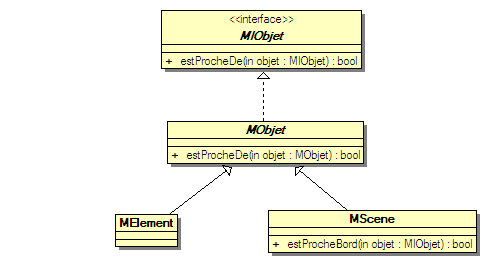
\includegraphics[width=1.0\textwidth]{uml/estProcheDe.png} 
			\\	
			\caption{Recherche de Proximité}
			\label{recherche_proximite}
		\end{center}
	\end{textblock*}		
 \begin{textblock*}{18cm}(2cm,16cm) 
	\subsubsection{Le test de collision de proximité}
		Nous avons choisi de réaliser le test de collision de proximité avec la méthode des axes séparateurs. Cette méthode s'appuie sur le théorème de l'axe séparateur:
		\begin{theoreme} \label{th_axe_separateur}
	Pour deux polyèdres convexes P et P', disjoints, il existe un axe A sur lequel la projection des polyèdres P  et P' forme deux intervalles disjoints. \\ 
\indent Un tel axe est appelé axe séparateur.\\

\indent Si les polyèdres sont disjoints, il existe un axe séparateur orthogonal à:
			\begin{itemize}
				  \item une face de P,
				  \item une face de P',
				  \item une arête de chacun des deux polyèdres.
			\end{itemize}
		\end{theoreme}
		
		La méthode des axes séparateur consiste donc à:
		\begin{itemize}
			  \item déterminer tous les axes séparateurs potentiels entre les deux figures
			  \item vérifier s'il en existe un sur lequel les projections des deux figures sont disjointes
			  \item si un tel axe n'existe pas signaler la collision et renvoyer l'axe selon lequel la collision est arrivée
		\end{itemize}
		\\
\end{textblock*}
\newpage
\indent Voici une illustration de deux formes convexes en collision, on remarque bien que les projections des deux formes se chevauchent:\\
		\begin{center}
			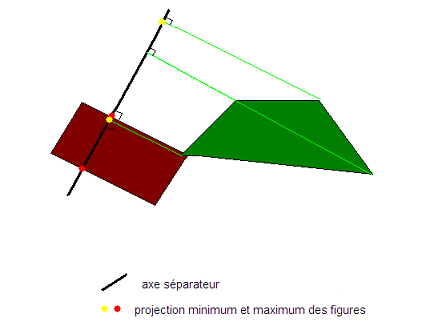
\includegraphics[width=0.7\textwidth]{img/polygone-collision.png} 
			\\		
			\caption{Exemple de polygones en collision}
		\end{center}
		\label{polygone-collision}
		\\
	\indent Si en revanche les deux formes ne sont pas en collision, les deux projections sont disjointes:
		\begin{center}
			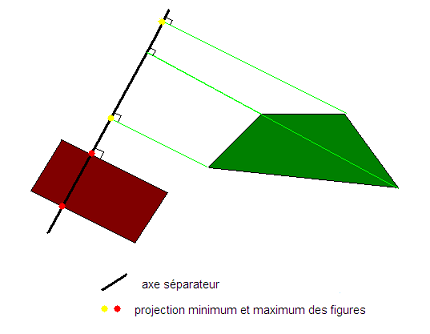
\includegraphics[width=0.7\textwidth]{img/polygone-non-collision.png} 
			\\		
			\caption{Exemple de polygones sans collision}
		\end{center}
		\label{polygone-non-collision}
		\\
	\indent Pour notre projet, c'est la fonction \textit{axeCollision(forme:MIForme)} implémentée dans MForme qui fait cela. Elle récupère les axes séparateurs des deux formes grâce à la méthode \textit{getAxesSeparateurs(forme:MIForme)} et demande à chaque forme de se projeter dessus grâce à la fonction \textit{seProjeteSur(vecteur:MVecteur)}. Cette fonction récupère les points à projeter avec la fonction \textit{getPointsProjection(axe:MVecteur)} et retourne les valeurs minimales et maximales des deux projections.\\ 
	\indent Si les deux projections sont disjointes, l'axe est séparateur et donc la fonction s'arrête là et renvoie null.\\
	\indent S'il n'y a pas d'axe séparateur alors la fonction retourne l'axe sur lequel le chevauchement des projections était minimal, c'est selon cet axe que les deux formes se sont percutées.
	\begin{textblock*}{18cm}(2cm,5cm)
		\begin{center}
			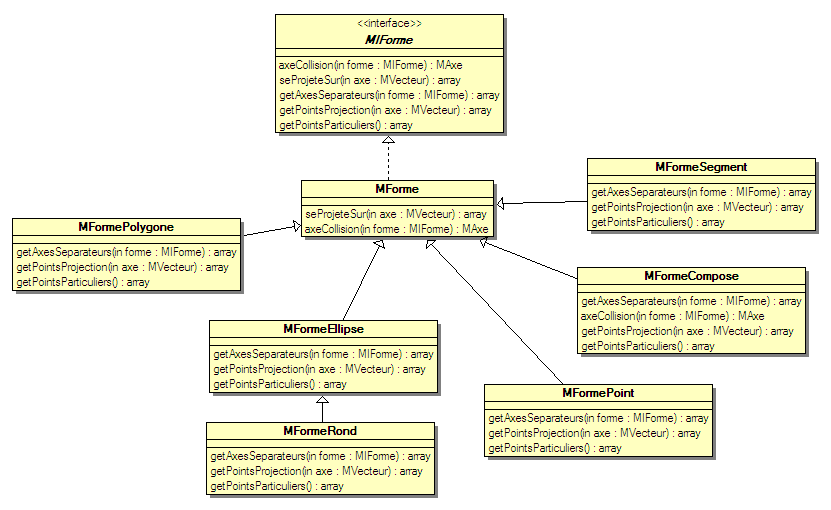
\includegraphics[width=1.0\textwidth]{uml/axeCollision.png} 
			\\		
			\caption{Test de collision de proximité}
		\end{center}
		\label{test_collision}	
		\\
	\end{textblock*}	
\newpage
	 \indent A cette méthode générale s'ajoute un certain nombre de cas particuliers:	
		\begin{enumerate}
			\item fonction \textit{getPointsProjection(axe:MVecteur)} :
				\begin{description}
					\item [ Les polygones:] Les points à projeter sont évidemment les sommets qui composent le polygone.
					\item [ Les formes ronds:] Les points à projeter pour les formes rondes sont les points d'intersection entre le rond et l'axe séparateur.
					\item [ Les formes composées:] L'ensemble des points à projeter pour une forme composée est l'union des points à projeter pour chacune des formes qui la compose.
				\end{description}
			\item fonction \textit{getAxesSeparateurs(forme:MIForme)} :
				\begin{description}
					\item [ Les formes polygones et les formes Segments:] Les axes séparateurs potentiels pour les polygones sont comme l'indique le théorème les axes qui sont perpendiculaires à ses arêtes. Pour le segment, c'est aussi l'axe qui lui est perpendiculaire. 
					\item [ Les formes ronds et les formes points:] Les formes ronds et les formes points n'ayant pas d'arêtes, les axes séparateurs ne peuvent être les perpendiculaires aux arêtes. Heureusement, les axes potentiels pour les formes ronds et les points sont les droites qui relient les points retournés par sa méthode getPointsParticuliers() à ceux de l'autre forme. Pour les ronds les points particuliers sont le centre, pour un point, c'est lui même, pour les polygones, ce sont ses sommets et pour une forme composée l'ensemble de ses points particuliers est l'union des points praticuliers des formes qui la compose. Donc par exemple, les axes séparateurs potentiels entre un rond et un triangle sont les axes qui relient le centre du cercle à chacun des sommets du triangle.
					\item [ Les formes composées:] L'ensemble des axes séparateurs pour une forme composée est l'union des axes séparateurs de chacune des formes qui la compose.
				\end{description}
			\item fonction \textit{axeCollision(forme:MIForme)} :
				\begin{description}
					\item [ Les formes composées:] Pour détecter la collision dans une forme composée, il faut détecter la collision dans chacune des formes qui la compose. Si aucune d'elles n'est en collision alors la forme composée n'est pas en collision
				\end{description}
		\end{enumerate}


	\subsection{Le jeu}
		Une fois les éléments du jeu mis en place il peut être intéressant de pouvoir les lancer et les stopper à bon escient. Notre framework possède une classe MJeu -qui est un singleton- permettant de lancer et de stopper les mouvements d'une scène quand celle ci le décide.
		\\
		\indent En effet à tout moment une scène peut récupérer l'instance du jeu et se placer en tant que scène principale de celui-ci. Elle peut donc demander quand elle le souhaite de lancer le jeu ou de le stopper ce qui aura pour effet de lancer les mouvements des éléments dans la scène ou de les arrêter. Par exemple si l'on souhaite un jeu avec un compte à rebours, il suffit de lancer un timer et au bout de ce timer demander au jeu de s'arrêter et de stopper tout. Ou encore si l'on fait un casse brique, on peut vérifier à tout moment la présence de brique dans la scène et continuer ou arrêter le jeu selon.
		\\
		\indent Pour finir le jeu permet en plus de compter un ou plusieurs scores, pratique pour les jeux multijoueurs.

\newpage
\section{Contrôleur}
Le rôle du contrôleur dans le modèle MVC est de recevoir les événements de l'utilisateur et de lancer les actions qui en découlent. Pour les jeux d'arcades, les événements qui nous intéressent principalement sont les événements de la souris et les événements du clavier sur l'ensemble de l'application. Nous avons donc défini deux classes chargées de prévenir les objets écouteurs inscrits dans leur liste des événements de l'application.

	\subsection{Souris}
% mélanie
	\indent La classe MSouris est un singleton, elle s'enregistre auprès de l'application pour les événements de clic, de double-clic et de déplacement de la souris. Elle retransmet ensuite à ses écouteurs les actions de clic, de double-clic et de déplacement vers le haut, bas, gauche, droite de la souris grâce à un calcul sur les coordonnées de l'évenement de déplacement. Les MIEcouteurSouris ont donc pour chaque événements une fonction qui contient le code à effectuer lors de l'événement et que MSouris appelle quand il faut.\\
	\begin{center}
		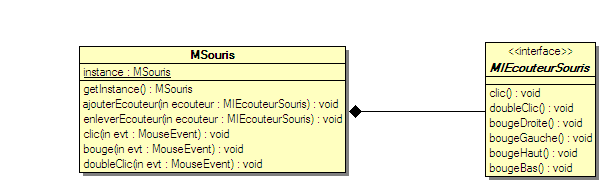
\includegraphics[width=1.0\textwidth]{uml/souris.png} 
		\\		
		\caption{La gestion des événements souris de l'application}
	\end{center}
	\label{souris}	
	\\
		
	\subsection{Clavier}
% mélanie
	La classe MClavier est aussi un singleton, elle s'enregistre auprès de m'application pour les événements d'appui de touche. Dans la fonction appui elle regarde quelle touche est appuyée pour pouvoir appeler la fonction adéquate de ses écouteurs. Les touches flèche haut, bas, gauche, droite, espace et entrée ont une fonction particulière dans les écouteurs car ce sont les touches les plus utilisées pour les jeux, pour les autres touches, une fonction commune est appelée avec en paramètre le code numérique de la touche et c'est au programmeur de différencier les touches	appuyées s'il en a besoin. \\
	\begin{textblock*}{18cm}(1cm,20cm)
		\begin{center}
			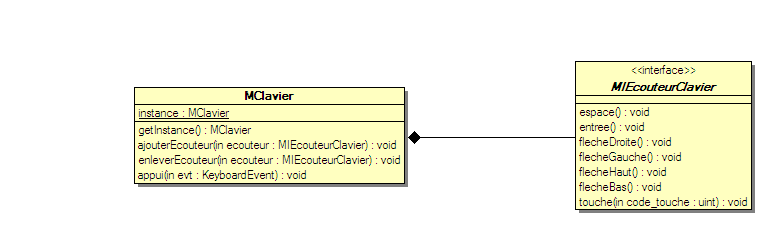
\includegraphics[width=1.0\textwidth]{uml/clavier.png} 
			\\		
			\caption{La gestion des événements claviers de l'application}
		\end{center}
		\label{clavier}	
	\end{textblock*}
	\\
\newpage
	\subsection{Effets}
% mélanie
	Les effets sont l'ensemble des traitements nécessaires pour créer l'illusion d'actions comme le mouvement, le changement de taille... Un effet s'applique sur un objet MIObjet, il utilise un timer pour fournir 50 changements par seconde et donner ainsi l'impression de continuité de l'effet.\\
  	\indent Il y a deux types d'effets, les effets à effectuer sur un temps fini ou les effets à effectuer de manière infinie. Par exemple, un mouvement peut être un déplacement jusqu'à un point en un temps donné ou un mouvement selon une direction et une vitesse avec rebondissement lorsqu'un obstacle est rencontré.\\
	\indent Pour les effets finis, au lancement de l'effet, on calcule les modifications à faire sur l'objet toutes les unités de temps ( pour obtenir 50 images/seconde, l'unité de temps est de 20 ms) puis on lance le timer le nombre de fois qu'il faut pour finir l'effet. \\
	\indent Pour les effets infinis le principe est le même sauf que l'on lance le timer un nombre de fois infinis. \\
\\
	\indent Voici notre hiérarchie d'effets:
	\begin{textblock*}{17cm}(1cm,13cm)
		\begin{center}
			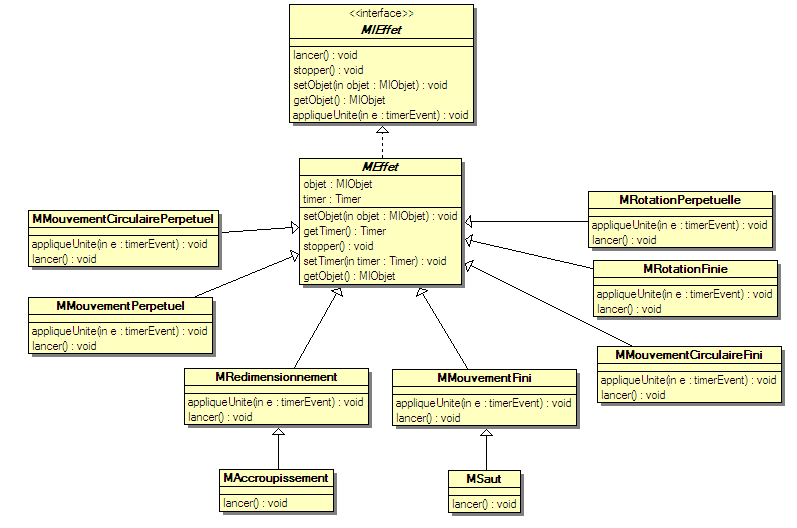
\includegraphics[width=1.1\textwidth]{uml/effet.png} 
			\\		
			\caption{Les effets}
		\end{center}
		\label{effet}	
	\end{textblock*}

\newpage
\section{Graphique}
La première chose que voit un joueur lorsqu'il joue à un jeu vidéo est le graphisme. Malgré que le plus gros travail ait été apporté au coeur de notre framework, nous avons voulu qu'un programmeur puisse créer simplement des objets qui sont graphiquement complexes. En effet, un jeu qui a un très bon gameplay et/ou un très bon concept ne sera pas utilisé, si celui-ci à un graphisme peu attrayant.
\\ \\
\indent Puisque nous utilisons l'API flex d'Adobe pour ce framework, nous avons dû nous limiter à ce qu'il peut nous offrir. Et comme dans toute API graphique, celle d'adobe est très complète mais son utilisation et implémentation reste bien souvent assez mystérieuse.

	\subsection{Réutilisation des composants de flex}
		\begin{center}
			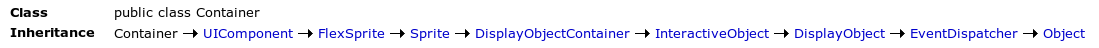
\includegraphics[width=1.1\textwidth]{img/flexHeritage.png}
			\caption{Héritage dans l'API 3.5 de flex}
		\end{center}		
\\
Lorsque nous avons fini de mettre en place notre code métier, il nous a fallu pouvoir afficher quelque chose. Pour cela nous avons essayé plusieurs composants qu'ils soient conteneur ou contenu. 
Puisque nous avons créé un framework entier et que notre code métier prend en compte tous les calculs, il nous a paru évident d'utiliser des composants de plus haut niveau possible, afin de ne pas surcharger inutilement notre framework avec des fonctions hérités de l'API qui deviendraient inutiles. Ainsi nous avons trouvé des composants de type DisplayObject qui sont les premiers composants affichables dans la hiérarchie de l'API de flex.
\\ \\
\indent En outre nous voulons que nos utilisateurs puissent écrire leur code, non seulement en ActionScript3, mais aussi en mxml. Pour cela nous avons dû descendre un peu dans la hiérarchie pour aller chercher UIComponent. Cette classe est donc notre point d'entrée dans l'API d'adobe. Ce composant permet d'ajouter des UIComponent dans un UIComponent, ce qui est pratique pour notre Pattern Composite du code métier entre les MScene et les MElements. Malheureusement nous perdrions la programmation mxml car on ne peut pas ajouter d'enfants dans un UIComponent en mxml, nous sommes donc encore descendu dans la hiérarchie pour représenter nos MScene, et le conteneur Canvas est celui de plus haut niveau qui permet l'ajout d'un enfant en mxml. De plus, il nous permet de positionner nos objets en absolu.
\\ \\
\indent Ensuite, le plus compliqué a été de comprendre comment fonctionne les UIComponent. Après avoir effectué de multiples recherches et encore plus de tests nous sommes finalement arrivés à cerner le fonctionnement interne de cette classe. En effet, à chaque fois qu'un UIComponant doit être affiché à l'écran, la fonction updateDisplayList est appelée. Nous l'avons donc tout naturellement réimplémentée.
	
	\subsection{Dessiner en ActionScript}

	%\begin{textblock*}{19cm}(1cm,3cm)  
		\begin{center}	
			\centering	
			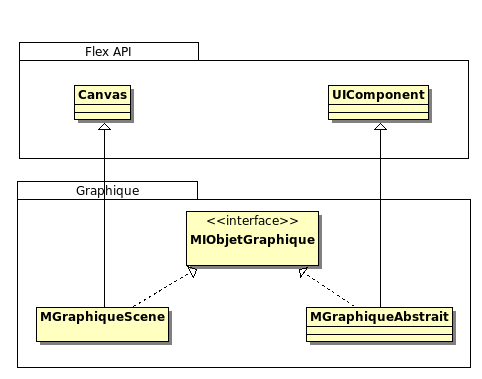
\includegraphics[width=1.0\textwidth]{img/UML-MUS-D-Flex.png}
			\caption{Hiérarchie entre notre graphisme et celui de Flex}
		\end{center}	
	%\end{textblock*}

\indent Par le biais de l'héritage dans nos classes graphiques, et l'attribut graphics, qui est le point d'entrée pour tout ce qui concerne le dessin en ActionScript, nous pouvons dessiner à l'écran des rectangles, des ellipses mais aussi des lignes. De plus flash nous permet de colorier nos formes avec de la couleur et des dégradés. Enfin il nous a paru intéressant de pouvoir ajouter des images et des textes dans nos formes, nous devrons utiliser d'autres classes mais le tout doit rester invisible pour le programmeur qui utilise notre framework.
\\ \\
\indent Une hiérarchie peut donc être mise en place, nos différentes formes seront dessinées par les classes graphiques les représentants alors que les textures devront pouvoir être appliquées à toutes ces formes.

\newpage
\\
	\begin{textblock}{19cm}(1cm,)
		\begin{center}
			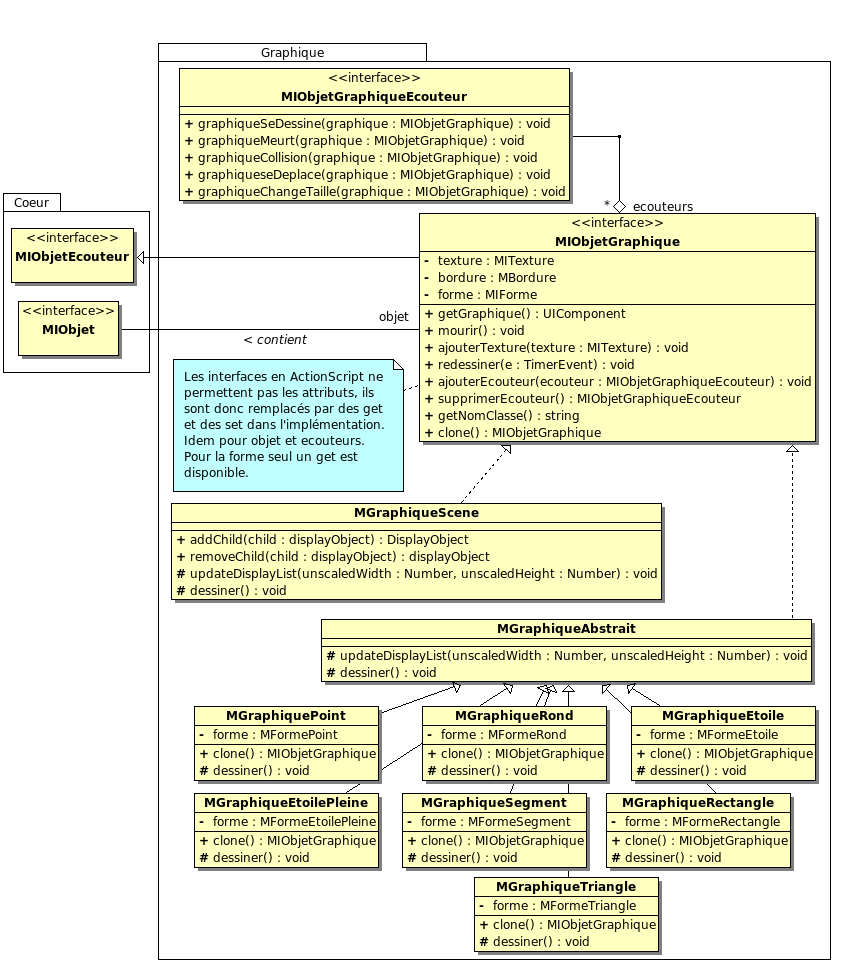
\includegraphics[width=1.0\textwidth]{img/graphiqueUml.png}
			\caption{Diagramme UML de la partie graphique}
		\end{center}
		%\label{cas_utilisation}
	\end{textblock}
\newpage
\subsection{Liaison avec le code métier}

Comme nous pouvons le voir la classe MGraphiqueAbstrait est la classe abstraite qui s'occupe de la relation entre l'API flex, le code métier et le programmeur. En effet celle-ci permet de positioner l'objet au travers des fonctions setX et setY, mais aussi de positionner la taille de l'objet avec les fonctions setWidth et setHeight. Ces fonctions sont des réimplémentations des fonctions de la classe UIComponent, elles doivent donc se mettre en accord avec l'API flex, pour qu'il continue d'afficher ces objets mais aussi et surtout ces fonctions doivent mettre à jour notre modèle afin que la détection de la collision puisse continuer.
\\ \\
\indent Ayant fait le choix d'utiliser le patron de conception Model-Vue-Controleur (plus communément appelé MVC) pour notre framework, il a tout naturellement fallu positionner la Vue (donc le graphisme) comme écouteur du modèle. Ainsi lorsque le modèle se déplace ou se redimenssionne, le graphisme en est prévenu et l'image vue par l'utilisateur correspond au model de notre framework. Les fonctions citées plus haut ont eu juste à faire passer l'information au modèle, ainsi le graphisme se remet à jour puisqu'il est écouteur du modèle.

	\subsection{Textures et le pattern "decorator"}

	%\begin{textblock*}{19cm}(1cm,3cm)  
		
		\begin{center}
			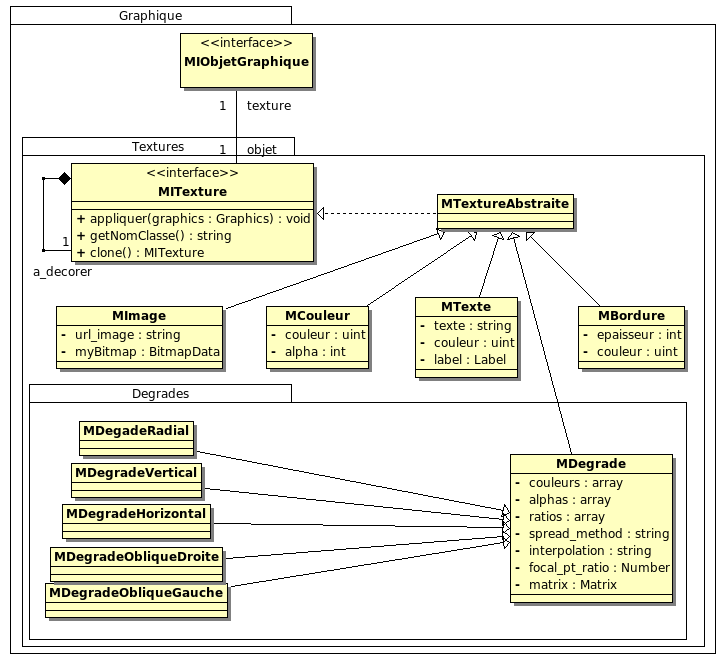
\includegraphics[width=1.1\textwidth]{img/graphiqueTextureUml.png}
			\caption{Diagramme UML des textures}
		\end{center}
		%\label{cas_utilisation}
	%\end{textblock*}

\indent Le dernier point de la partie graphique de notre framework est la texture d'un objet. En effet, une fois que nous avions réglé le problème de la forme il nous a fallu réfléchir au moyen de lui donner une texture. De base Flex nous permet de colorier une forme avec une couleur ou un dégradé. Pour plus de facilité nous permettons à l'utilisateur de créer des dégradés horizontaux, verticaux, radiaux mais aussi obliques. De plus nous souhaitions pouvoir mettre une image en tant que texture d'un objet. Pour cela nous avons dû charger l'image dans une matrix (pixel par pixel) avant de pouvoir dessiner cette matrix sur l'objet en question. Enfin la technique est à peu près similaire pour pouvoir poser un texte comme texture, mais cette fois, nous utilisons le fait qu'un UIComponent puisse contenir des enfants. Pour cela nous stockons le texte dans un Label avant de l'ajouter à l'objet. Malheureusement en agissant ainsi nous ne pouvons pas cacher le texte dépassant de la forme.
\\ \\
\indent Enfin, pour que l'on puisse ajouter un texte ou une image par dessus une couleur ou un dégradé nous avons mis en place un patron de conception Décorateur. Ainsi nous pouvons ajouter à une forme autant de textures que l'utilisateur le souhaite. Puisque le flash gère très bien la transparence des couleurs, toutes les possibilités sont permises non seulement dans le code mais aussi et surtout à l'affichage.

	\subsection{Les écouteurs du graphisme}

\indent Après avoir commencé à programmer quelques jeux nous nous sommes rendus compte que le fait de devoir étendre systématiquement les classes graphiques pour pouvoir faire interagir les objets était trop contreignant. Partant de cela, nous avons décidé de placer des écouteurs également dans la partie graphique. Ainsi le programmeur qui souhaite pouvoir faire rebondir une balle, sans forcément réimplémenter la classe MGraphiqueRond, peut simplement l'écouter. Il sera alors prévenu lorsque la balle se déplace, se redimensionne ou encore lorsqu'elle collisionne. Comme vous pouvez le constater il s'agit d'un exemple et tous nos objets graphiques fonctionnent sur le même principe.
\\ \\
\indent Ainsi, le programmeur a deux choix pour pouvoir agir sur ses objets graphiques. Le premier étant d'étendre l'une des classes graphiques, il lui faudra alors penser à appeler super() dans les fonctions de MIObjetGraphiqueEcouteur pour appeler les fire. Le deuxième étant de simplement écouter un objet en ajoutant la classe qui implémente MIObjetGraphiqueEcouteur dans les écouteurs de l'objet à surveiller.

\newpage
	\section{Patron de conception Fabrique}
	Puisque le programmeur a à sa disposition tous ces éléments et qu'il va vouloir les représenter graphiquement par toutes nos formes, nous avons naturellement pensé à utiliser le patron de conception Fabrique.

	\begin{center}
		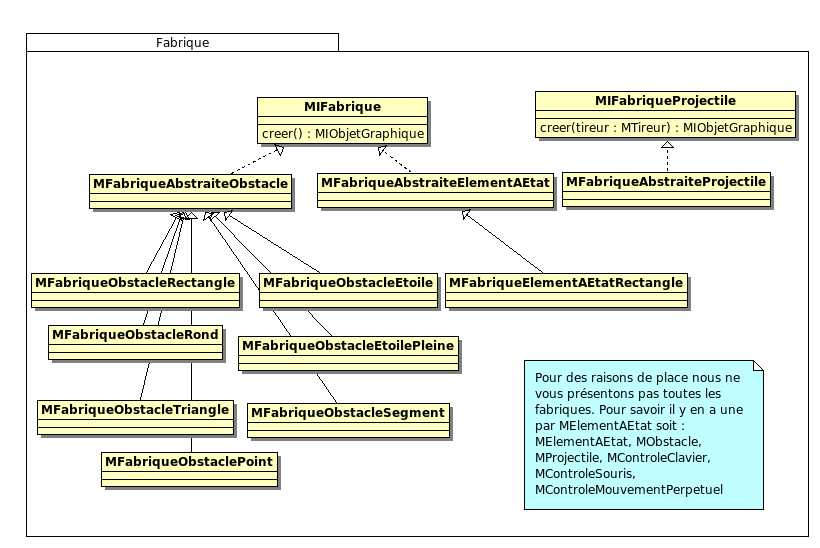
\includegraphics[width=1.00\textwidth]{img/Fabrique.png}
		\caption{Diagramme UML de la fabrique}
	\end{center}
\\
	\indent Comme vous pouvez le voir nous avons mis en place plusieurs fabriques pour que l'utilisateur puisse de façon transparente conjuguer les éléments avec les différentes formes. Grâce aux fabriques l'utilisateur dispose de plusieurs choix pour remplir ses scènes. En effet il peut le faire de manière "traditionnelle" en instanciant un MIObjetGraphique qui, de base créé un MElement (l'élement de plus haut niveau), puis en lui positionnant l'objet modèle qu'il souhaite (en appelant setObjet(objet)). Ou alors il peut faire appel à une de nos fabriques pour créer un MProjectile (qui est un MElementAEtat) rond par exemple. L'interface MIFabrique permet de rendre les classes MFabriqueAbstraite[TypeElement] abstraite, puisque action script 3 ne le permet pas.
\\
	\indent Le schéma nous montre aussi que chaque fabrique possède plusieurs fonctions pour créer les objets en question. En effet, il nous a paru nécessaire de pouvoir créer simplement tous types d'éléments, mais aussi et surtout de pouvoir en créer avec le plus de détails possible. De plus, la plupart du temps nous avons opté pour une fonction de création par défaut qui initialise les objets avec des valeurs de base (surtout utile pour le débuggage). Nous avons également programmé une fonction qui permet de créer les objets en détaillant leur côté modèle, puis une autre fonction détaillant le graphisme et une dernière fonction qui mèle les deux côtés.


\newpage
\section{Créateur de jeu}
	Tout comme son nom l'indique le créateur de jeux est un logiciel permettant de créer facilement des jeux vidéos de types arcade. L'objectif du départ était de créer un logiciel avec lequel on pourrait créer un jeu en quelques clics, nous avons finalement produit un logiciel dans lequel il suffit de glisser les différents objets qui constitueront le jeu et de leur associer une texture, un  ou plusieurs types de mouvement et de contrôle, puis de générer le code qui constituera le jeu. L'aide concernant l'utilisation du logiciel se trouve dans l'annexe de ce rapport.
	\subsection{Utilisation du framework}
	\indent Le framework a été très utile pour confectionner le créateur de jeux. Dans cette image vous pouvez voir les types d'objets du framework que nous avons utilisés : \\
	
	\begin{center}
		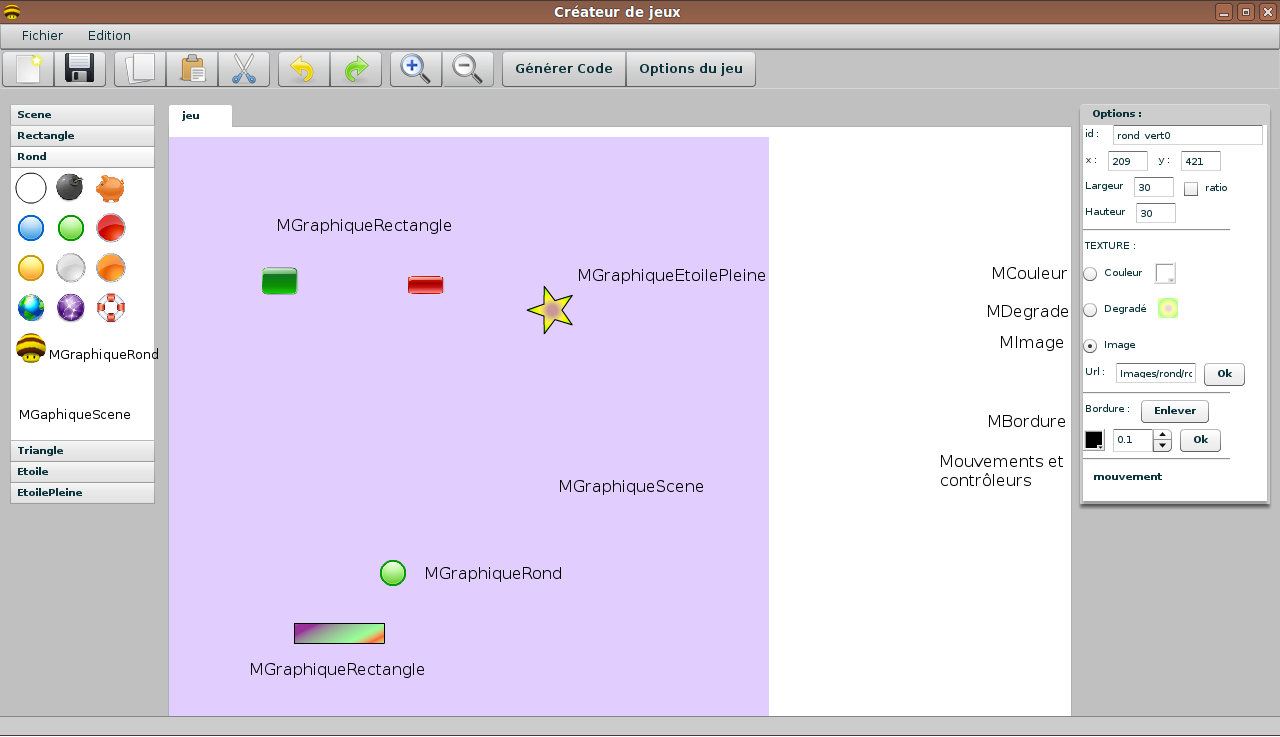
\includegraphics[width=1.1\textwidth]{img/createurJeux.png}
		\caption{Créateur de jeux }
	\end{center}
		\subsubsection{Créations des formes}
	Afin d'offrir à l'utilisateur un maximum de formes aux textures différentes, nous avons décidé de proposer des MIObjetGraphique dont les textures seraient des images toutes prêtes (avions, murs...). \\
	\indent Il a cependant fallu trouver un moyen simple de les représenter et de les stocker. Le framework propose plusieurs types de formes telles que rectangle, triangle ou encore étoile. Nous avons donc choisi de placer les images de créateur de jeux en fonction de ces formes. Ainsi, l'utilisateur peut choisir le type d'objet qu'il veut utiliser en fonction de sa forme. Pour cela, il a fallu que l'on trouve un moyen simple de stocker toutes ces images, nous avons alors créé un fichier xml dont chaque noeud représente le nom d'une classe graphique du framework (ex: MGraphiqueRectangle, MGraphiqueTriangle...), avec des noeud enfants représentant les images qui lui sont associées et dont l'url pointe vers une image présente dans les sources du projet. \\
	\indent Ainsi, il nous suffit de parser ce fichier et pour chaque noeud père nous avons créé un menu-accordéon qui contient une MGraphiqueScene sur laquelle on positionne chacun de nos objets en leur associant pour texture une MImage dont le chemin se situe dans le fichier xml. \\
	\indent Dans la fonction de parsage, nous appelons une fonction qui prend en paramètre un string qui correspond à un nom de classe de notre framework et qui retourne une instance de cet objet. De cette façon, si le noeud père est MGraphiqueRectangle, nous créons un menu-accordéon au nom de Rectangle qui ne contiendra que des objets de type MGraphiqueRectangle. \\
	\indent Le fait d'utiliser un fichier xml construit de cette façon, permet à l'utilisateur de rajouter facilement des images adaptées à ces objets en complétant simplement ce fichier. De plus, dans le cas où l'utilisateur aurait créé un nouveau type de MIObjetGraphique, il n'aurait plus qu'à compléter de la même manière le fichier. L'aide concernant la modification du fichier xml, se trouve dans l'annexe de ce rapport. Lorsque flex permettra d'enregistrer des fichiers sur l'ordinateur de l'utilisateur, une extension possible du créteur de jeux serait une interface graphique permettant de rajouter des images au fichier xml plus simplement.
		\subsubsection{L'onglet central}
	L'onglet central est une MGraphiqueScene, c'est ici que l'utilisateur pourra créer son jeu. De plus, il aura la possibilité de changer le type de texture de la scène grâce au panel d'option situé sur la gauche. \\
	\indent Pour créer un jeu, il suffit simplement de placer des objets sur la scène et de leur donner une action. Nous utilisons le mécanisme du drag\&drop pour ce qui concerne le déplacement des objets du menu-accordéon vers la scène. Lors du drop, nous utilisons la méthode clone() d'un MIObjetGraphique. Ainsi, les objets du menu-accordéon sont conservés, et on crée un nouvel objet dans la scène qui possède les mêmes propriétés que celui du menu-accordéon. \\
	\indent Le framework ayant été construit sur le modèle MVC, lors d'un ajout dans la scène du côté graphique, le modèle est mis à jour automatiquement, ainsi dans le créateur de jeux, lors d'un drop, nous ne nous préoccupons pas du côté modèle de la scène. 
		\subsubsection{Modifications des propriétés d'un objet}
	 Afin que l'utilisateur puisse modifier le plus possible les objets comme s'il le faisait en programmant, nous avons installé un panel d'options contenant toutes les actions qu'il peut réaliser pour modifier les propriétés d'un objet. Ainsi, quelque soit le type de MIObjetGraphique il peut changer :
	\begin{itemize}
 		\item la taille de l'objet
		\item sa position sur la scène
		\item sa texture : MCouleur, MDegrade, MImage
		\item rajouter ou enlever sa bordure
		\item lui ajouter un ou plusieurs types de mouvements
		\item lui associer un type de contrôle : souris et/ou clavier
		\item lui associer ou modifier son id (identifiant)
	\end{itemize}

	\indent De plus, et toujours grâce au modèle mvc, dès qu'une modification de ce panel est effectuée, elle se répercute immédiatement sur le modèle et sur le graphisme, on peut ainsi voir en direct les modifications réalisées.

		\subsubsection{Génération de code}
	Afin que l'utilisateur qui créé son jeu puisse pouvoir le tester, il faut qu'il génère le code de son application. Nous n'avons pas pu intégrer de compilateur flex/actionScript à notre créateur, donc il faut compiler les sources du jeu en passant par Eclipse. De plus, nous ne pouvons pas enregistrer le code que nous produisons avec le créateur, car flex ne le permet pas. De ce fait, nous ne pouvons pas sauvegarder ni restaurer ce que fait l'utilisateur. Pour parer à ce manque, lors de l'appui sur le bouton \textit{GénérerCode}, nous ouvrons une fenêtre qui contient le code, et nous proposons à l'utilisateur de copier tout le code par le biais d'un bouton destiné à ça.  \\
	\indent Nous générons un code flex, donc à balises, pour tout ce qui concerne la création des objets et leur propriétés, et un code de type \textit{script} pour associer des écouteurs aux objets. Nous générons également les classes pour les différents écouteur : effets, claviers, souris.\\
		\subsubsection*{Mécanisme de génération du code}
	\indent Comme nous l'avons vu précédemment, à chaque fois qu'un objet est ajouté à la scène, supprimé, ou modifié, le modèle est lui aussi modifié, grâce au MVC. Afin de générer du code, nous parcourons simplement la liste des enfants de la scène et pour chacun d'entre eux, nous parcourons la liste de ses textures, de ses mouvements et de ses types de contrôle. En fonction de tous ces paramètres, nous générons le code qui lui correspond. De plus, si l'utilisateur ajoute un mouvement ou un type de contrôle, la classe correspondante est elle aussi automatiquement générée. \\
	\indent Il suffit alors que l'utilisateur copie tout le code dans Eclipse, et qu'il rajoute les différentes actions qu'il souhaite donner à ses objets.
		\subsection{petite conclusion}
	Le créateur de jeux a été programmé en même temps que le framework, il a permis notamment de pouvoir tester les différentes texures, mais aussi de mettre en évidence des problèmes de programmation qui ont été réglés par la suite.

\newpage	
\section{Jeux}
% john
Nous avons décidé de faire un premier jeu qui servira d'exemple aux futurs utilisateurs de notre framework.
Pour cela nous avons choisi un jeu qui utilise beaucoup de fonctionnalités. Il s'agit d'une forme
de Ping-pong.
	\subsection{Le Menu}
Pour commencer, nous avons fait un menu principal qui permettra de naviguer dans le jeu, modifier les commandes,
voir les règles... 
\begin{center}
	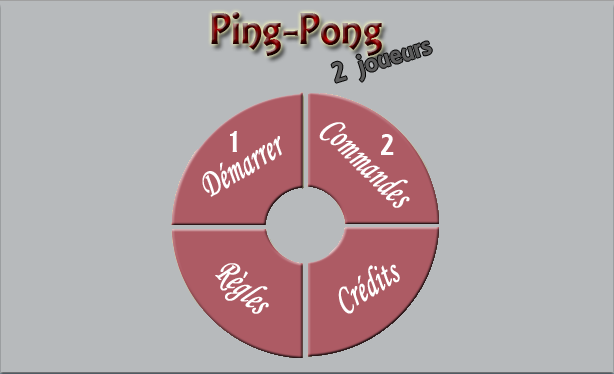
\includegraphics[scale=1.00]{img/menu.png}
\end{center}
\indent Il s'agit donc d'une simple \textit{MGraphiqueScene} dans laquelle on a ajouté des boutons. Ces boutons ont été personnalisés grâce à un fichier css externe. Il a suffi de rajouter des actions sur le clic. \\

Légende:
\begin{enumerate}
	\item Démarre le jeu en affichant la MGraphiqueScene du jeu
	\item Affiche la MGraphicScene des Commandes
\end{enumerate}

	\subsection{Les Commandes}
Ce panneau de commande permet aux deux joueurs de personnaliser leurs commandes et ce quelque soit
le moment. En effet, en pleine partie, l'utilisateur peut accéder à ce panneau.
\begin{center}
	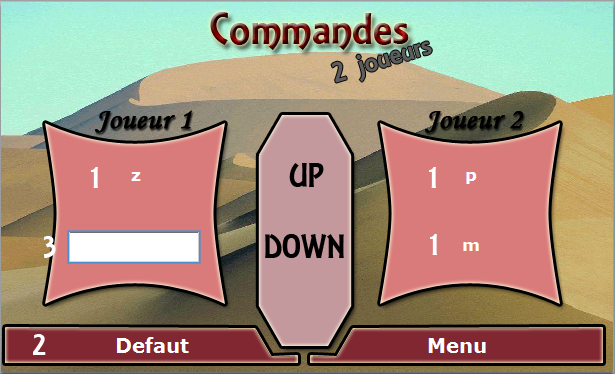
\includegraphics[scale=1.00]{img/commandes.png}
\end{center}
\\
\indent Il s'agit donc d'une simple "MGraphiqueScene" dans laquelle on a ajouté deux boutons personnalisés. Il y a également des "MImage", des "Label", et des "Textfield". Il a suffi de rajouter des actions sur le clic des boutons et des "Label", ainsi que des actions sur les touches (KeyEvent).\\ \\
Le principe est le suivant:
\begin{enumerate}
	\item On clique sur un label d'une touche
	\item Cela ouvre un Textfield sur ce label
	\item Puis l'utilisateur appuie sur une touche
	\item La touche est reconnue puis le label se réaffiche avec pour texte cette nouvelle touche
\end{enumerate}
\\ \\ 
\indent Légende:
\begin{enumerate}
	\item Label qui lors du clic affiche le textfield
	\item Textfield affiché après le clic sur le label
	\item Bouton permettant de remettre les commandes par défaut
\end{enumerate}

\subsection{Le Jeu}
Le panneau du jeu est le plus complexe. Mais le framework a vraiment simplifié les choses comme on le verra ultérieurement. Il s'agit d'une MGraphiqueScene contenant plusieurs élements graphiques. Certains sont en mouvement grâce à des événements claviers, d'autres sont en mouvement perpétuel et d'autres sont statiques. \\
\indent La balle est un MGraphiqueRond avec une MTexture qui permet de lui mettre une image de fond ainsi qu'une MBordure permettant de mettre une bordure autour de la balle.  \\
\indent Ce MGraphiqueRond implémente MIObjetGraphiqueEcouteur ce qui permet de réimplémenter certaines méthodes telle que graphiqueCollision(...). Celui-ci contient également un MMouvementPerpetuel qui permet notamment de gérer par exemple les trajectoires.\\
\begin{center}
	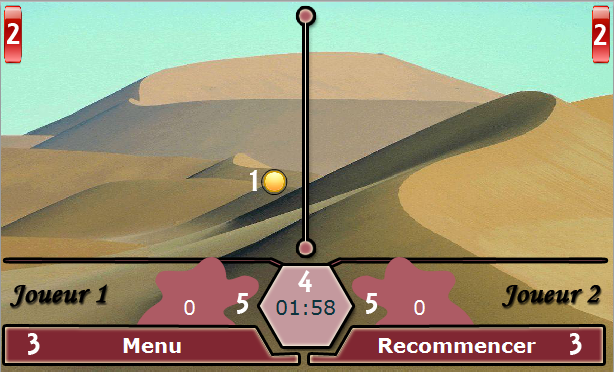
\includegraphics[scale=1.00]{img/jeux.png}
\end{center}

Légende:
\begin{enumerate}
	\item La balle qui traverse la MGraphiqueScene
	\item Les raquettes qui font rebondir la balle
	\item Boutons permettant de recommencer la partie ou de retourner sur le menu
	\item Timer affichant le temps restant
	\item Points de chaque joueur
\end{enumerate}

\subsection{Les données}
Ce jeu a été d'une grande aide au fur et à mesure de l'avancée du framework. Il a permis d'identifier différents bugs tant au niveau graphique que modèle. Le fait d'avancer le jeu en même temps que le framework a donné des idées supplémentaires pour simplifier la programmation de petits jeux d'arcades. \\ \\
Le Ping-Pong réunit les statistiques suivantes:
\begin{itemize}
	\item Création des différentes images et boutons peronnalisés: 2 Jours
	\item 5 classes: Menu, Jeu, Commandes, Balle, Raquette
	\item Moins de 900 lignes de codes
	\item Peut être implémenté en une journée si la personne à une bonne connaissance du framework
\end{itemize}

\newpage
\section{Conclusion}
	Les fonctionnalités dont on parle dans l'introduction ont été implémentées dans notre framework, ainsi, grâce à notre framework, un utilisateur peut maintenant créér facilement un jeu d'arcade, à condition bien sûr qu'il ait quelques notions de programmation. Il pourra ainsi publier son jeu sur internet, ou l'utiliser en application de bureau. De plus grâce aux MElement que nous avons rajouté, un utilisateur peut facilement créer des éléments ayant un comportement particulier comme par exemple un petit personnage qui pourrait tirer des missiles, s'accroupir et sauter.\\
	\indent Nous avons utilisé de nombreux patrons de conception, ce qui fait que notre framework est facilement extensible, un utilisateur pourra donc facilement étendre notre framework à sa guise pour fabriquer par exemple de nouvelles formes, de nouvelles textures, ou de nouveaux mouvements, et ce en rajoutant simplement des classes dans notre hiérarchie. \\
	\indent Nous avons développé ce framework dans l'optique de l'utiliser pour programmer nos propres jeux d'arcades, ainsi, les principales fonctionnalités que nous avons implémenté sont apparues naturellement au cours de la programmation des jeux. \\

	\subsubsection{Difficultés}
	\indent Comme vous pouvez le constater, tout le nécessaire à la création d'un jeu d'arcade est présent dans notre framework, cependant, nous aurions par exemple pu améliorer la gestion des ellipse. Nous avons une classe qui gère les ellipses, mais nous avons remarqué que la façon de traiter la collision pour ce type de forme était très complexe, nous avons alors décider de ne pas continuer de développer les ellipses. De plus, nous avons commencé à programmer des formes complexes composées d'autres formes, elles mêmes pouvant être complexes, mais par soucis de temps, nous avons préféré privilégié le développement des éléments plutôt que de continuer à élaborer les formes complexes. Il serait également possible de rajouter d'autres éléments ou d'autres actions. Néanmoins, le framework est utilisable puisque grâce à lui nous avons pu créer facilement : un jeu de ping-pong, un jeu de type "Space invader" et un "pac-man". \\

	\subsubsection{Connaissances acquises}
	\indent Ce projet nous a apporté de nombreux bénéfices, tout d'abord, nous avons appris comment faire un framework, et surtout comment organiser nos classes afin qu'elles soient extensible et utilisables facilement. Ainsi, nous avons utilisé de nombreux patrons de conception, et le fait de les avoir implémenté nous a imposé une certaine rigueur dans notre programmation, le modèle MVC a également été d'une grande aide pour rendre notre programmation plus clair. \\
	\indent Ce projet a été réalisé en groupe, et nous a donc appris à travailler en groupe, à réfléchir ensemble, et surtout à programmer ensemble. L'utilisation de logiciels de SVN, ou du site googleCode a été d'une grande aide pour partager nos idées et notre travail. \\
	\indent Nous avions choisi de programmer en utilisant l'API flex. Nous ne connaissions pas les langages de l'API qui sont MXML et l'ActionScript, cela a d'abord été un léger frein dans le développement du framework, mais nous nous sommes énormément documentés et ces langages étant très intuitifs, nous avons réussi à comprendre ces mécanismes et à les maîtriser. Dans la partie bibliographie, nous vous fournirons les divers liens vers les sites internet qui nous ont été utiles. \\
\indent Nous avons également créé un site internet sur lequel nous avons mis : les sources de notre projet ainsi que les jeux et le créateur de jeux, qui sont accessibles en ligne à l'adresse suivante : http://mus-d.lydiman.net/.

\section{Bibliographie}
	\subsection{Général}
	\begin{itemize}
		\item http://fr.wikipedia.org
		\item http://www.adobe.com/livedocs/flex/3/html/index.html
		\item http://www.adobe.com/devnet/flex/tourdeflex/web/
	\end{itemize}
	\subsection{Collision}
	\begin{itemize}
		\item http://www.flashxpress.net/ressources-flash/la-detection-de-collision/
		\item http://www.javafr.com/codes/COLLISIONS-2D-AXES-SEPARATEURS\_42788.aspx
	\end{itemize}	
	\subsection{Contrôleur}
	\begin{itemize}
		\item http://blog.flash-actionscript.com/actionscript-3-les-ecouteurs-d-evenements/
	\end{itemize}	
	\subsection{Créateur de jeux}
	\begin{itemize}
		\item http://examples.adobe.com/flex2/consulting/styleexplorer/Flex2StyleExplorer.html
	\end{itemize}
	
\newpage
\section{Annexe}

\subsection{Guide pour l'utilisation du créateur de jeux}
	\begin{center}
		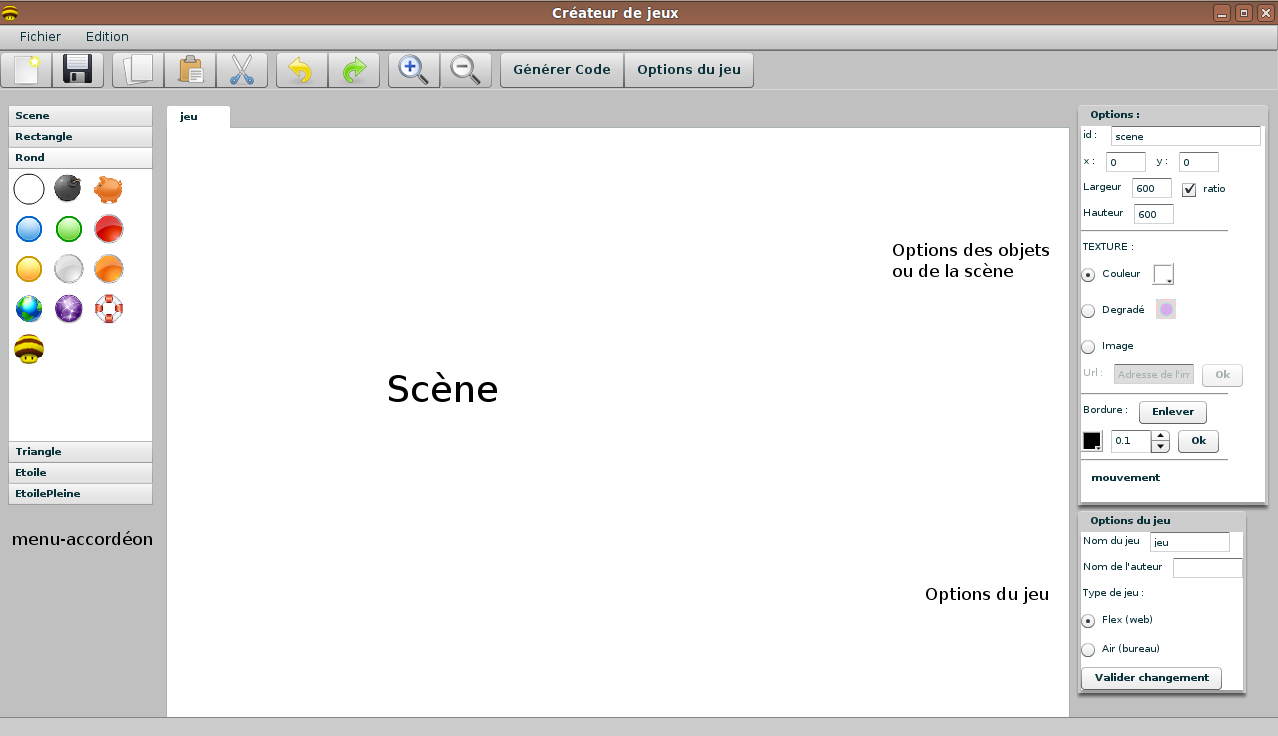
\includegraphics[width=1.00\textwidth]{img/createurjeu.png}
	\end{center}
	\subsubsection{Création d'un premier jeu}
	Dès l'ouverture du logiciel, il est possible de créer son premier jeu dans l'onglet central qui est en fait la scène du jeu. Néanmoins, on peut également faire \textit{Fichier -> Nouveau} ou cliquer sur la barre d'outil pour créer un nouvel onglet et ainsi créer un nouveau jeu, ou un nouveau niveau. Après avoir cliqué sur \textit{Fichier->Nouveau}, une fenêtre s'ouvre demandant à l'utilisateur de choisir un nom pour son jeu, d'entrer le nom de l'auteur et de choisir le type de jeu qu'il désire. En effet, l'utilisateur a la possibilité de choisir si il veut créer un jeu à publier sur Internet, et pour cela il doit cocher la case Flex, ou si il veut créer une application de bureau, et dans ce cas il devra cocher la case Air, l'utilisateur aura à tout moment la possibilité de modifier ce choix. Tous les choix réalisés dans cette fenêtre seront utiles dans la génération du code, le titre apparaîtra dans l'onglet du navigateur web, ou dans la barre de titre de l'application bureau. Ces différents choix seront modifiables tout au long de la création du jeu, et ce en appuyant sur le bouton : \textit{Options du jeu} ou en cliquant sur la scène de fond. Après avoir validé, un nouvel onglet apparaît, et l'utilisateur peut alors créer un autre jeu. Chaque onglet représente un nouveau jeu, ou un nouveau niveau.
	\begin{textblock*}{14cm}(4cm,21cm)
		\begin{center}  
			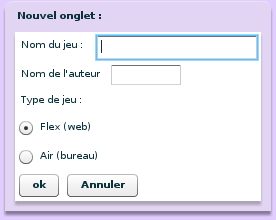
\includegraphics[width=0.5\textwidth]{img/nouvel-onglet.png} 
		\end{center}
	\end{textblock*}
\newpage	
	\subsubsection{Ajout des éléments à la scène}
	Après avoir ouvert un onglet, l'utilisateur peut alors positionner des objets qui seront des éléments de son jeu. Afin d'ajouter des éléments à la scène, l'utilisateur doit simplement choisir un des objets contenus dans le menu-accordéon situé sur la gauche, puis de le glisser à l'aide de la souris sur la scène à la position de son choix. L'utilisateur peut ajouter autant d'éléments qu'il le souhaite, et ce aux endroits qu'il désire. \\
\indent L'utilisateur peut également utiliser le copier/coller pour copier un objet qui serait déjà présent sur la scène, pour ce faire, il doit utiliser les raccourcis clavier : \textit{ctrl-c} et \textit{ctrl-v} (seulement dans la version bureau de l'application) ou alors les boutons prévus à cet effet dans la barre d'outil. \\
\indent Dans le cas où un utilisateur voudrait supprimer un objet de la scène, il peut également le faire, en appuyant sur la touche \textit{suppr} de son clavier.
	
	\subsubsection{Modification des propriétés des objets}
	L'utilisateur peut modifier autant qu'il le souhaite les objets qui sont présents dans la scène. Tout d'abord, il doit cliquer sur un objet en particulier afin de lui donner le focus, dès lors, un carré rouge se met autour de l'objet pour signifier qu'il est sélectionné, et toutes les informations relatives à cet objet s'inscrivent dans le panel d'options (situé sur la droite). L'utilisateur peut alors modifier tous les champs de ce panel, il a la possibilité de modifier : 
	\begin{itemize}
		\item l'identifiant de l'objet,
		\item sa position en x et en y, l'objet se place en fonction de ce que l'utilisateur entre comme paramètres,
		\item sa largeur et sa hauteur, il peut choisir de garder le ratio, donc la proportion entre la largeur et la hauteur, ou de ne pas le garder et ainsi, cela pourra par exemple modifier la forme de l'objet (un carré peut ainsi devenir un rectangle),
		\item sa texture : la couleur grâce à un ColorPicker, le dégradé, ou l'image en entrant le chemin vers l'image
		\item lui ajouter ou enlever une bordure
		\item lui affecter un ou des mouvements, des contrôleurs
	\end{itemize}	
	\begin{textblock*}{14cm}(4cm,17cm)
		\begin{center}
			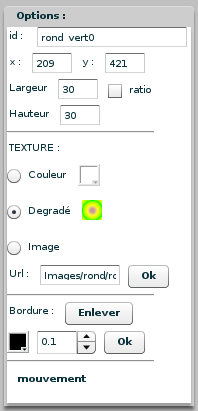
\includegraphics[scale=0.7]{img/option.png}
		\end{center}
	\end{textblock*}
\newpage
		\subsubsection*{Modification du dégradé}
%% copie d'écran du panel dégradé
	En cliquant sur \textit{Dégradé}, une fenêtre s'ouvre permettant de créer un nouveau dégradé. Elle propose de régler toutes les options nécessaires à instancier un MDegrade. Malgrés tous les choix dont dispose l'utilisateur, la création d'un nouveau dégradé est assez intuitive. \\
		\begin{center}
			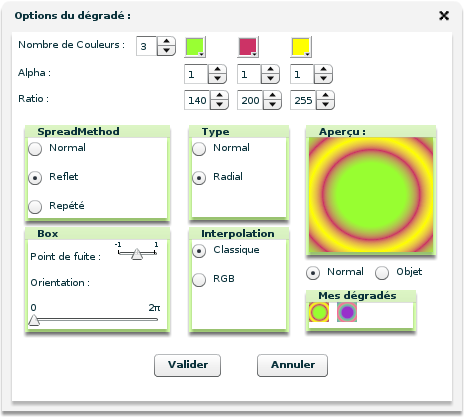
\includegraphics[scale=0.7]{img/degrade.png}
		\end{center}
\indent Le panel d'option \textit{SpreadMethod} permet de choisir le type de diffusion du dégradé : normal, répété, ou en reflet. \\ 
\indent Le panel \textit{type} permet de choisir si le dégradé sera normal, ou radial. \\
\indent Le panel \textit{Box} sert à définir le point de fuite du dégradé, dans le cas où il serait radial, et son orientation. La modification de l'orientation permet de créer des dégradés verticaux, obliques, horizontaux, en fonction d'un angle choisi grâce au slider. \\
\indent La fenêtre de dégradé propose également une MGraphiqueScene dans laquelle on peut voir un aperçu du dégradé, en cliquant sur \textit{objet}, l'utilisateur aura un aperçu de son dégradé appliqué à son objet. Après avoir validé, le dégradé est appliqué à l'objet, et le dégradé créé est ajouté à la liste des dégradés préférés de l'utilisateur.
\newpage
		\subsubsection*{Ajout d'effets, de contrôleur}
	En cliquant sur le bouton \textit{Mouvement}, une fenêtre permettant de choisir les différents mouvements et contrôles apparaît. 
		\begin{center}
			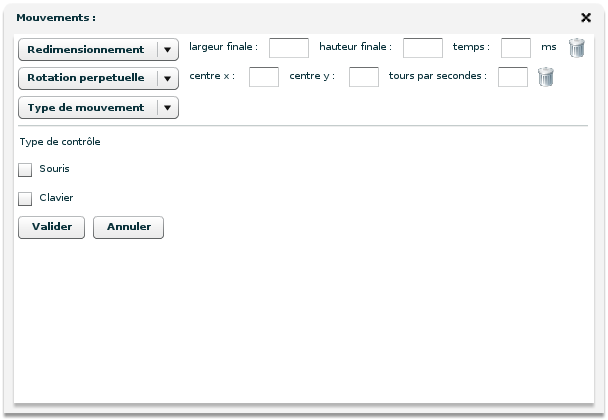
\includegraphics[scale=0.7]{img/mouvement.png}
		\end{center}
\indent L'utilisateur peut tout d'abord choisir le type de mouvement à appliquer à son objet : perpétuel, fini, ou redimensionnement. Dès lors qu'il fait son choix, les différentes options du mouvement s'affichent à l'écran, ainsi, en fonction du mouvement l'utilisateur doit choisir : 
	\begin{itemize}
		\item mouvement perpétuel : l'angle de lancement de départ, et la vitesse de l'objet
		\item mouvement fini : la valeur du x et du y d'arrivée, et le temps pour réaliser cette action, en milliseconde
		\item redimensionnement : la largeur et la hauteur finale, et le temps pour réaliser cette action.
		\item circulaire fini : le point autour du quel l'objet va tourner, l'angle et le temps en milliseconde
		\item circulaire perpétuel : le point autour du quel l'objet va tourner, le nombre de tour par seconde qu'il va réaliser
		\item rotation perpétuelle : le point autour du quel l'objet va tourner, le nombre de tour par seconde qu'il va réaliser
	\end{itemize}
	L'utilisateur peut ajouter autant de mouvements qu'il le souhaite. Il seront ensuite traités dans la génération du code. \\
	\indent Afin d'ajouter un type de contrôleur pour son objet : clavier ou souris, il suffit qu'il coche la ou les cases correspondantes.
\newpage
		\subsubsection{Génération du code}
	En appuyant sur le bouton \textit{Générer code}, une fenêtre contenant le code de l'application permettant de la lancer est générée. \\ 
		\begin{center}
			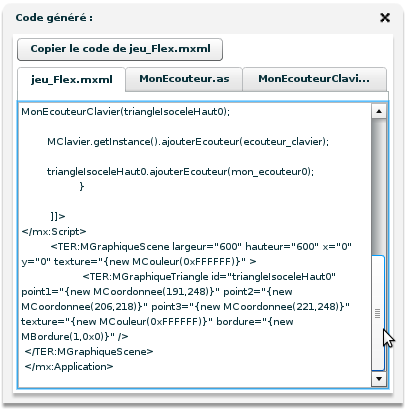
\includegraphics[scale=0.7]{img/code.png}
		\end{center}
\indent Dans le cas où les objets auraient des mouvements ou des contrôleurs, nous générons également le squelette des classes contenant les méthodes des interfaces à réimplémenter. L'utilisateur n'aura alors qu'à compléter ces fichiers. Nous produisons des classes qui implémentent les écouteurs : MIObjetGraphiqueEcouteur, MIEcouteurSouris et MIEcouteurClavier. \\ \indent Cette fenêtre est composée de plusieurs parties : un éditeur de texte contenu dans un onglet, chaque onglet correspondant à la génération du code de l'application et/ou des classes à réimplémenter, et d'un bouton permettant de copier tout le code de l'onglet dans le presse papier.

		\subsubsection{Utilisation du code généré}
	Flex ne permet pas d'enregistrer, de modifier ou d'ouvrir des fichiers qui se trouvent sur l'ordinateur de l'utilisateur, donc pour qu'il puisse utiliser le code généré par l'application, il doit :
		\begin{itemize}
			\item Ouvrir Eclipse
			\item Créer un nouveau projet flex ou air, en fonction du type de jeu qu'il souhaite créer.
			\item Coller le code de l'application dans le fichier \textit{.mxml}
			\item Coller le code des classes dans des classes actionScript portant le même nom
			\item Coller les différentes images qui constituent le jeu
			\item Implémenter les différentes fonctions du comportement des objets
			\item Compiler le projet avec Eclipse
			\item Lancer le jeu
			\item Jouer !
		\end{itemize}
		
		\subsubsection{Ajouter des éléments au menu-accordéon}	
	L'utilisateur peut facilement ajouter des éléments au menu-accordéon, il suffit pour cela qu'il modifie le fichier xml appelé \textit{liste\_image.xml}. \\
	\indent Dans le cas où l'utilisateur voudrait ajouter des objets à un menu déja existant, il doit simplement rajouter une ligne au fichier, à l'endroit où se trouve le noeud de la classe de l'objet à rajouter. Par exemple, si il souhaite ajouter un rectangle dont l'image est marron, il doit alors compléter le noeud "MGraphiqueRectangle". \\
	\indent Si en revanche l'utilisateur crée un nouveau type d'objet, il devra alors rajouter un nouveau noeud, dont le nom sera celui du nouveau type. \\ \\
	\indent Voici un exemple de noeud : \\
<MGraphiqueRectangle>\\
   <carre id="carre\_bleu" source="Images/carres/bleu.png" largeur="64" hauteur="64"/>
</MGraphiqueRectangle> \\

	\\
Voici ici un exemple générique d'un noeud du fichier : \\
<NomDeLaClasseGraphique> \\
   <classe id="mon\_id"  -- paramètres nécéssaires à la création des objets -- /> \\
</NomDeLaClasseGraphique>

\end{document}
